%!TEX root = ../main.tex

The use of mobile broadband for accessing the Internet via tablets and smartphones has increased rapidly as a result of high speed mobile networks, such as 3G and 4G. The web browsers on these devices are becoming more and more similar in capabilities to their desktop versions. It is possible to run \gls{wrtc} applications in some of them, and these features will become more available with time. This section is going to look at the use of \gls{wrtc} in mobile devices. We start by looking at some of the issues we have to deal with when working with mobile devices, then we will look at performance and quality metrics derived from current research.

\subsection{Network performance}
It is feasible to run \gls{wrtc} applications on mobile devices. However, battery consumption, persistent connectivity, and quality performance remain a big challenge. A lot of work is being done in radio technologies, but the most important factors are how the applications, protocols, and API's are designed\cite{isomaki2012considerations}. First we will look at some of the performance issues of serving wireless video.

The most used and relevant networks are Wi-Fi, WiMAX, and the different telecommunication networks. Serving wireless video is a significant challenge for already-stressed cellular data networks\cite{erman2011over}. Video traffic requires high bandwidth, imposes latency and packet loss. The key is to deliver video as high in quality as the network supports. By looking at a study testing video and audio quality on two differenet WiMAX networks\cite{fund2013performance}, we can see variations of performance in two different locations.

\pagebreak
\begin{figure}[here]
\centerline{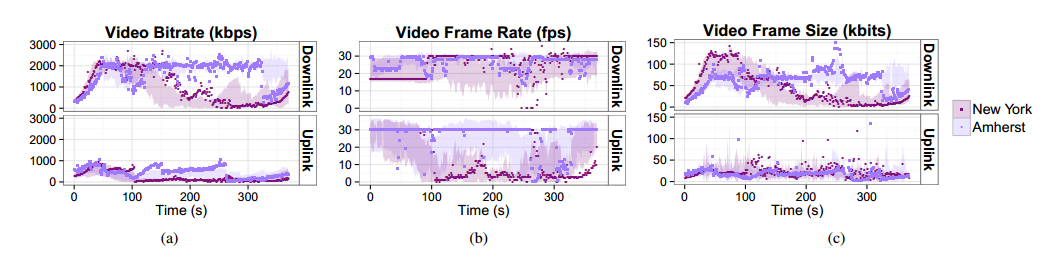
\includegraphics[width=\textwidth]{mobile-video-metrics.png}}
\caption{WebRTC video performance. Adapted from: Performance of DASH and WebRTC Video Services for Mobile Users\cite{fund2013performance}.}
\label{fig:mobile-video-metrics}
\end{figure}

\gls{wrtc} adapts to changing link conditions by estimating the available sent bandwidth and passing this estimate to the encoder as a target bitrate. Figure \ref{fig:mobile-video-metrics} show key metrics of video and audio quality for a \gls{wrtc} session sustained over a WiMAX link in two different locations. The color blue is a suburban setting (Amherst) and purple is an urban setting (New York). For each plot, the shaded area shows one standard deviation above and below the mean, while the points give values for a representative trial. These values are presented from the perspective of the mobile WiMAX-connected peer. There is a dramatic difference in performance between the two locations, with the suburban setting always outperforming the urban setting. The uplink stream has significantly worse video performance than the downlink. This is probably due to the asymmetry of the cellular link. Only 25\% of radio resources are allocated to the uplink\cite{fund2013performance}. A result of this is a reduced frame rate, this is unfortunate since mobile users are often walking, which makes the video feed have a high motion content.

\pagebreak
\begin{figure}[here]
\centerline{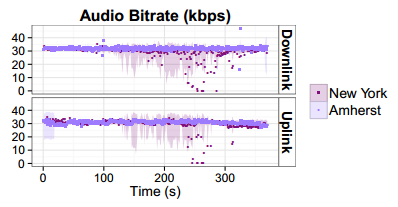
\includegraphics[scale=0.55]{mobile-audio-metrics.png}}
\caption{WebRTC audio performance. Reprinted from: Performance of DASH and WebRTC Video Services for Mobile Users\cite{fund2013performance}.}
\label{fig:mobile-audio-metrics}
\end{figure}

An important thing to mention is that video quality is not that important when it comes to communication, the audio quality is of much more value\cite{fund2013performance}. In Figure \ref{fig:mobile-audio-metrics} audio performance is shown as representative values (points) and a range of one standard deviation above and below the mean (shaded area). We can observe that the audio bitrate is mostly consistent, degrading only in extremely poor channel quality. The biggest problem here as seen in Table \ref{tbl:wrtc-packet-loss} is that the packet loss is quite high on the uplink for audio in the urban environment. This is because the quality is not reduced to keep the audio signal clear. This could be somewhat fixed by retransmission of the packets, but this will again increse latency.
\\
\begin{table}[here]
\centerline{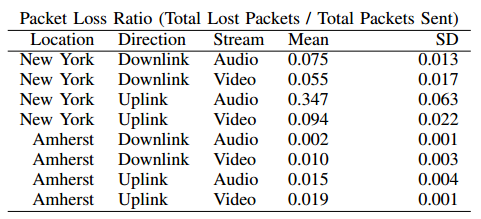
\includegraphics[scale=0.5]{wrtc-packet-loss}}
\caption{Packet loss ratio for a WebRTC session. Adapted from: Performance of DASH and WebRTC Video Services for Mobile Users\cite{fund2013performance}.}
\label{tbl:wrtc-packet-loss}
\end{table}

\subsection{Connectivity}
Another concern is persistent connectivity. For an app to be reachable for incoming connections, it needs some kind of persistant communication channel. Most cellular networks have a firewall preventing incoming TCP connections\cite{isomaki2012considerations}. To keep a TCP connection alive, the application needs to send some kind of keep-alive packets with a high enough frequency to avoid a connection timeout. Problem with keeping a connection open all the time, is that the device's radio will consume a lot of battery. %herefore, the keep-alive packets should only be sent infrequently.

\subsection{Summary}
Most of the performance issues is handled by the underlying technologies of \gls{wrtc}, which actually is pretty good at adapting bandwidth usage in variable network conditions. But it is important to be aware of these problems, when developing applications. The effect that a mobile users uplink is much worse than it's downlink has great impact on a user's perception of the connection. However, the most important factor for us to consider is how we will do the signaling with a mobile device, since we can't keep a connection open all the time, as that would drain the battery.